\documentclass[12pt,a4paper]{article}
\usepackage[width=.75\textwidth]{caption}
\usepackage{graphicx}
\usepackage{authblk}
\usepackage{amsmath}
\usepackage{amsfonts}
\usepackage{braket}
\usepackage{epigraph}
\usepackage{amssymb}
%\usepackage{mathrsfs}
\usepackage[mathscr]{euscript}
\usepackage[top=2cm, bottom=2cm, left=2cm, right=2cm]{geometry}
\usepackage{fancyhdr}


\setlength{\epigraphwidth}{0.8\textwidth}

\pagestyle{fancy}
\begin{document}

%title and author details
\title{Multi-Observer Quantum Mechanics from Classical Bayesian Inference}
\author[1]{Kevin Player\footnote{kjplaye@gmail.com}}

\maketitle


\epigraph{I would not call [entanglement] {\bf one} but rather {\bf the} characteristic trait of quantum mechanics, the one that enforces its entire departure from classical lines of thought.}{Erwin Schrödinger}

\abstract{We present several quintessential quantum ideas and shed them in a classical light.  The ideas presented all have analogues in classical information theory.  For instance, entanglement is presented as a generalization of classical correlation.  We argue how quantum information theory can be understood as a generalization of classical information theory in a nonstandard way (without density matrices).  In fact, we show how classical information theory can be embedded in quantum information theory as zero phase wavefunctions.  We employ this embedding to motivate a new multi-observer version of quantum mechanics. Finally, we outline an experiment to test the existence of our multi-observer theory.}

\section{Some Thought Experiments}
Lets start with a 3-bit example, where each bit is realized by coins which are heads (H) or tails (T).  With these 3 coins in hand, we conduct some thought experiments.
\subsection{Configurations}
Let us try to describe the situation once we throw the 3 coins.  Let
\[
x_i \in \{H,T\}
\]
be the outcome for the throws $i$ = $1,2,3$ and let $x$ be the resulting configuration sequence.  Nominally, we have 3 ``dimensions'' worth of information to describe the 3 coins.  Lets move on and generalize.
  
\subsection{Classical Information Theory}
In the following subsections we outline an epistemic treatment where we try to represent our knowledge of the 3 coin ensemble. We want to describe a general knowledge statement about the coins.  We will build this up here using basic probablistic statements and classical superpositions.

For any configuration $x$ we have the knowledge statement $b_x$, that says we know $x$ with probablity 1.  We call this a basic statement.  There are 8 configurations, so there are 8 basic statements.

A classical superposition can be made for any probabilistic statements $s_1$ and $s_2$ and $\alpha \in [0,1]$
\[
\text{super}_\alpha(s_1,s_2) = \alpha s_1 + (1 -\alpha) s_2.
\]
This is statement $s_1$ with probablity $\alpha$ and statement $s_2$ with probability $(1-\alpha)$.  Repeatedly applying superpositions starting with the basic statements and then also to the resulting substatements allows us to consider knowledge statements as general probability distributions on the ensamble of coins.

\subsubsection{Distributions on the Ensamble}
The general knowledge statements on 3 coins are in fact an 8 dimensional space spanned by the 8 basic statements
\[
   p_0,\cdots,p_{7} \in \mathbb{R}^+
\]
and normalized with $\sum p_i = 1$.  Each $p_i$ is the probability of the coins being in a configuration state given by the binary expansion of $i$.  For instance $p_5$ is the probability of seeing $THT$. Notice that we have not moved to quantum information theory, but we are already motivated to use 8 dimensions instead of 3.

\subsubsection{Bayesian Projections as Classical Wave Function Collapse}
\label{proj}
We don't always get to measure the exact configuration.  For instance, we might only get to know that the first coin is $T$ and that the 2nd and 3rd coins are the same.  This corresponds to an exemplar subset of $\{0,\cdots,7\}$, which we will call
\[
\begin{split}
  S &= \{s \in \{0,\cdots,7\} | c_1(s) = T, c_2(s) = c_3(s) \} \\
    & = \{4,7\} \hspace{0.4 in} \text{(THH, TTT)}
\end{split}
\]
where $c_i(s)$ is the value $x_i$.  Someone could make a measurement that tells them that the state is in $S$ and nothing else.  This would be a specific case of a projection measurement.  The wavefunction becomes zero exactly on $p_i$ where $i \not \in S$ and just renormalizes $p_i$ on the remaining $i \in S$.

\begin{figure}[h]
\centering
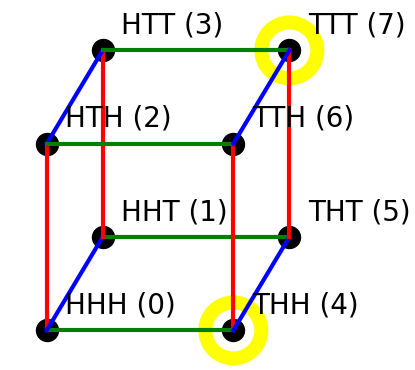
\includegraphics[scale=0.3]{cube.png}
\caption{Coin configurations with $S$ circled in yellow.}
\label{masslessshell}
\end{figure}


\subsubsection{Bayesian Inference as General Classical Wave Function Collapse}
A more general type measurement is a probabilistic measurement.  Someone could learn that there is a 95\% chance that the state is in $S$.  In full generality we will call such a probabilistic observation $\mathcal{O}$.  We can figure out how to update our knowledge statement from $p_i$, to $\hat{p_i}$, using a relative\footnote{In the ratio, the contribution of $P(\mathcal{O})$ is canceled out and accounted for during normalization.  $P(\mathcal{O})$ only holds significance prior to its observation and it doesn't require consideration during the update process.} version of Bayes's rule
\[
  \frac{\hat{p_i}}{\hat{p_j}} = \underbrace{\frac{P(i | \mathcal{O})}{P(j | \mathcal{O})}}_\text{Posterior}
                              = \underbrace{\frac{P(\mathcal{O} | i)}{P(\mathcal{O}|j)}}_\text{Bayes Factor}  \hspace{0.07 in}  \underbrace{\frac{p_i}{p_j}}_\text{Prior}
\]
Pulling out the Bayes factor we find that we just multiply by the likelihood and re-normalize
\[
  \hat{p_k} =  P(\mathcal{O} | k) \hspace{0.07 in} p_k.
\]
A special case are projections $P(\mathcal{O} | k) \in \{0,v\}$, for some fixed value $v$, like the $S$ projection case in section \ref{proj}.  We call these Bayesian projections.

\subsubsection{Classical Correlation as Classical Entanglement}
Finally, we can also consider distributions such as the two coin distribution $p_0,p_1,p_2,p_3$
\[
p_i = 
\left\{
\begin{split}
\frac{1}{2} & \mbox{ if } i \in \{0,3\}\\
0 &\mbox{ else }
\end{split}
\right.
\]
We have $HH$ or $TT$ with equal probabilities.  If I give the first coin to Alice and the second coin to Bob then we have a classical correlation.  If Bob finds that the first coin is $T$ then we know that Alice will also find $T$.  The reduction is purely epistemic, it is the separate knowledge of Alice and Bob that is changing.  This should all seem very reasonable from every day experience; classical correlation is not weird.

\subsection{Quantum Information Theory}
\subsubsection{Classical to Quantum Embedding}
General quantum information\footnote{We are purposely leaving out density matrices and POVMs and just dealing with pure states.} about 8-qbits can be expressed as a wave function.
\[
   q_0,\cdots,q_{7} \in \mathbb{C}
\]
with $\sum |q_i|^2 = 1$.  The Born rule is ostensibly a map $q_i \rightarrow |q_i|^2 = p_i$ to classical probability.  Here we can instrument all of the classical information theoretic constructs by restricting the phase\footnote{We consider negative values as 180 degrees out of phase, so zero phase means non-negative real.} of $q_i$ to be zero.  We can map backward $p_i \rightarrow \sqrt{p_i} = q_i$; which commutes with the Born rule (subject to normalization):

{
\renewcommand{\arraystretch}{0.1}
\[
\text{(Quantum)} \hspace{0.3 in}
\mathbb{C}^n \begin{array}{c} \twoheadrightarrow \\ \hookleftarrow \end{array}
(\mathbb{R}_{\ge 0})^n
\hspace{0.3 in} \text{(Classical)} 
\]
}

So quantum information theory needs to generalize the classical.  In particular, quantum measurement and entanglement restrict to classical measurement and classical correlation for zero phase.

\subsubsection{Bayesian Projection}
We illustrate zero phase Bayesian projection with an example.

Within the embedding we define a projection operator $\pi$ which projects onto the space generated by the subset $S$, from the previous subsection
\[
\pi = \sum_{i \in S} \ket{i} \bra{i}.
\]
Then let $A$ be any operator with an eigenspace, with eigenvalue $\lambda$, equal to the image of $\pi$.  An observation of $\lambda$ would correspond to an application of $\pi$, which is a Bayesian projection in the classical picture.

\subsubsection{Bayesian Inference}
Consider, in the fashion of \cite{nielsenchuang}, a more general measurement with matrix $M_\mathcal{O}$ which is diagonal with entries
\[
   M_\mathcal{O}(i,i) = \sqrt{P(\mathcal{O} | i)}
\]
This implements classical Bayesian inference using zero phase wavefunctions.


\subsubsection{Entropy}
Von Neumann entropy is left out of this note since it is not a generalization of classical entropy in the manner presented here.  This is because the zero phase classical wavefunctions are pure states which all have zero Von Neumann entropy.

\section{Overview of the Generalization}

The quantum mechanical concepts mentioned in Section 1 are a direct generalization of their classical information theoretic analogs.  This is not to say that they are not weird, but to say that they need to be generalizations of the classical concepts.  Wave function collapsing should generalize Bayesian inference and classical measurement.  Entanglement should be a generalization of classical correlation.  This is enough to motivate new ways of doing quantum mechanics, which we will encounter in the next sections.

\subsection{Multi-Observer Quantum Mechanics}
We focus on quantum wave function collapse as a generalization of classical Bayesian inference.  We can implement the classical Bayesian inference within zero phase quantum mechanics as outlined above.  So the classical Bayesian theory has a direct tie in; that observation and measurement occur in tandem with a change in knowledge\footnote{This change in knowledge is tangible, it always occurs as a transfer of matter/energy from the environment to the observer \cite{thrust}.}.  

In the classical theory, knowledge is local to the observer\footnote{Note that current quantum theory is a theory of one observer, usually the experimenter in a lab.  An immediate subject is quantum key distribution(QKD), which requires at least three observers, Alice, Bob, and Eve; the security of QKD depends on multi-observer quantum ontology.}, multiple observers each have their own knowledge.  For instance, Wigner's friend and Wigner each have their own classical knowledge.  It would seem then that Wigner's friend and Wigner must have different zero phase wavefunctions as well, if they are to be generalizing classical knowledge.  This is a prediction on multi-observer quantum physics, that every observer has a local wavefunction. 

\subsection{Prediction and Experiment}

We predict that multi-observer quantum mechanics will be required for a proper generalization of classical knowledge.  We propose an experiment where we inject an ``observer'' into a quantum eraser\footnote{Here we probe the boundaries of what constitutes an observer and a measurement.  We claim that all versions of observer and measurement will be detectable in this experiment whenever it can be done.}.  The injected observer will have to be a small apparatus that is
\begin{itemize}
   \item able to record a measurement $\psi$ of the eraser particle path.
   \item able to forget the measurement $\psi$.
   \item able to demonstrate that a measurement was made with a record $\rho$.
\end{itemize}
Let $\phi$ be the lab technician's wavefunction.  In $\phi$ the apparatus is entangled with the subject particles in the eraser experiment.  We need to find out if there is another wavefunction in play that is not just part of $\phi$.  The key here is that the apparatus is able to demonstrate that it ``knew'' something, or in other words that another wavefunction $\psi$ existed, using $\rho$.

The apparatus can not keep $\psi$ for proper erasure, but must ``forget'' it.  Observed erasure, via an interference pattern, proves that $\psi$ is not a part of $\phi$.  Finally, there should be a record $\rho$ in the apparatus that it did at one point in time record a measurement $\psi$.  Receipt of the report $\rho$ and eraser interference pattern together show that $\psi$ and $\phi$ were necessarily part of a two-observer system.

\section{Acknowledgments}
Thanks to Erik Ferragut and Dan Justice for useful discussions.

\bibliographystyle{ieeetr}
\bibliography{bibliography}

\end{document}
